\documentclass[UTF8,zihao=-4,a4paper]{ctexart}

\usepackage[left=2.25cm,right=2.25cm,top=2.30cm,bottom=2.35cm]{geometry}
\usepackage{amsmath,amssymb}
\usepackage{booktabs}
\usepackage{array}
\usepackage{tabularx}
\usepackage{longtable}
\usepackage{makecell}
\usepackage{multirow}
\usepackage{graphicx}
\usepackage{float}
\usepackage[section]{placeins}
\usepackage{caption}
\usepackage{xcolor}
\usepackage{enumitem}
\usepackage{fancyhdr}
\usepackage{microtype}
\usepackage{xurl}
\usepackage{hyperref}
\usepackage[most]{tcolorbox}
\usepackage{listings}
\usepackage{pdflscape}
\usepackage{threeparttable}
\usepackage[backend=biber,style=numeric,sorting=none,maxbibnames=6,giveninits=true]{biblatex}

\addbibresource{references_agent.bib}
\graphicspath{{../figures/}}
\newcommand{\FullContentMacroF}{86.49}
\newcommand{\FullOfficialMacroF}{87.75}
\newcommand{\FullOfficialDeltaPP}{1.26}
\newcommand{\FullOfficialDeltaLowPP}{0.58}
\newcommand{\FullOfficialDeltaHighPP}{1.94}
\newcommand{\SmallContentMacroF}{78.88}
\newcommand{\SmallRawMacroF}{61.69}
\newcommand{\SmallQwenMacroF}{80.75}
\newcommand{\SmallOfficialMacroF}{81.91}
\newcommand{\SmallDirectMacroF}{75.77}
\newcommand{\SmallQwenDeltaPP}{1.87}
\newcommand{\SmallQwenDeltaLowPP}{-2.80}
\newcommand{\SmallQwenDeltaHighPP}{6.69}
\newcommand{\SmallRawDeltaPP}{-17.19}
\newcommand{\RobertaMainContentMean}{87.16}
\newcommand{\RobertaMainContentSD}{0.45}
\newcommand{\RobertaMainOfficialMean}{88.30}
\newcommand{\RobertaMainOfficialSD}{0.08}
\newcommand{\RobertaMainDeltaPP}{1.13}
\newcommand{\RobertaSmallContentMean}{84.90}
\newcommand{\RobertaSmallQwenMean}{82.57}
\newcommand{\RobertaSmallQwenDeltaPP}{-2.34}
\newcommand{\QwenGenerationMeanSeconds}{0.562}
\newcommand{\QwenGenerationWallSeconds}{450.2}
\newcommand{\QwenGenerationPeakGiB}{6.40}
\newcommand{\QwenDirectMeanSeconds}{0.209}
\newcommand{\QwenDirectCoverage}{100.0}
\newcommand{\ContentOverlapPct}{14.44}
\newcommand{\ExactOverlapRows}{53}
\newcommand{\QwenTrainCrossContextPct}{81.00}
\newcommand{\QwenTestCrossContextPct}{99.50}

% Generated by make_improvement_assets.py; do not edit manually.
\newcommand{\ImproveTFIDFSmallContent}{78.88}
\newcommand{\ImproveTFIDFSmallOldConcat}{80.75}
\newcommand{\ImproveTFIDFSmallStructuredConcat}{80.84}
\newcommand{\ImproveTFIDFSmallOldLate}{82.39}
\newcommand{\ImproveTFIDFSmallStructuredLate}{80.03}
\newcommand{\ImproveTFIDFLargeContent}{82.29}
\newcommand{\ImproveTFIDFLargeStructuredConcat}{82.94}
\newcommand{\ImproveTFIDFLargeStructuredLate}{83.82}
\newcommand{\ImproveRobertaSmallContent}{84.90}
\newcommand{\ImproveRobertaSmallOldQwen}{82.57}
\newcommand{\ImproveRobertaSmallStructured}{82.44}
\newcommand{\ImproveRobertaSmallCompact}{84.30}
\newcommand{\ImproveRobertaSmallLateFusion}{84.88}
\newcommand{\ImproveRobertaLargeContent}{87.19}
\newcommand{\ImproveRobertaLargeStructured}{86.73}
\newcommand{\ImproveRobertaLargeCompact}{87.21}
\newcommand{\ImproveRobertaLargeLateFusion}{87.63}
\newcommand{\ImproveRobertaLargeLateDeltaPP}{0.43}
\newcommand{\ImproveRobertaSmallLateDeltaPP}{-0.03}
\newcommand{\ImproveTFIDFLargeLateDeltaPP}{1.53}
\newcommand{\ImproveTFIDFSmallOldLateDeltaPP}{3.51}
\newcommand{\ImproveTFIDFSmallOldLateLowPP}{-0.32}
\newcommand{\ImproveTFIDFSmallOldLateHighPP}{7.35}
\newcommand{\ImproveTFIDFLargeLateLowPP}{-1.28}
\newcommand{\ImproveTFIDFLargeLateHighPP}{4.34}
\newcommand{\ImproveQwenTestSmallCoverage}{99.50}
\newcommand{\ImproveQwenTrainLargeCoverage}{99.70}
\newcommand{\ImproveQwenTrainSmallCoverage}{99.75}


\definecolor{DeepBlue}{HTML}{484878}
\definecolor{MutedTeal}{HTML}{42949E}
\definecolor{SoftRose}{HTML}{C56A83}
\definecolor{LightBlue}{HTML}{EEF2F7}
\definecolor{LightRose}{HTML}{FAEEF1}
\definecolor{Ink}{HTML}{272727}
\definecolor{MutedGray}{HTML}{666666}

\hypersetup{
  colorlinks=true,
  linkcolor=DeepBlue,
  citecolor=MutedTeal,
  urlcolor=SoftRose,
  pdftitle={RTX 4060 上的 BC4RII 解释增强缩小复现实验},
  pdfsubject={Qwen3-8B、Chinese-RoBERTa 与直播弹幕推荐意图识别},
  pdfkeywords={BC4RII, Qwen3, GPU, explanation augmentation, recommendation intent}
}

\ctexset{
  section={format=\Large\bfseries\color{Ink},beforeskip=1.3ex,afterskip=0.8ex},
  subsection={format=\large\bfseries\color{DeepBlue},beforeskip=1.0ex,afterskip=0.5ex},
  subsubsection={format=\normalsize\bfseries\color{MutedTeal}}
}

\captionsetup{font=small,labelfont=bf,labelsep=quad,justification=centering}
\setlength{\parindent}{2em}
\setlength{\parskip}{0.22em}
\linespread{1.22}
\setlength{\emergencystretch}{2em}
\setlength{\headheight}{15pt}
\renewcommand{\arraystretch}{1.20}
\setcounter{tocdepth}{1}

\pagestyle{fancy}
\fancyhf{}
\fancyhead[L]{BC4RII 解释增强缩小复现实验}
\fancyhead[R]{RTX 4060 / Qwen3-8B}
\fancyfoot[C]{\thepage}
\renewcommand{\headrulewidth}{0.4pt}

\newtcolorbox{keybox}[1][]{
  enhanced,
  breakable,
  colback=LightBlue,
  colframe=DeepBlue,
  boxrule=0.6pt,
  arc=1.5mm,
  left=2.5mm,right=2.5mm,top=1.8mm,bottom=1.8mm,
  title=#1,
  fonttitle=\bfseries
}

\newtcolorbox{riskbox}[1][]{
  enhanced,
  breakable,
  colback=LightRose,
  colframe=SoftRose,
  boxrule=0.6pt,
  arc=1.5mm,
  left=2.5mm,right=2.5mm,top=1.8mm,bottom=1.8mm,
  title=#1,
  fonttitle=\bfseries
}

\lstset{
  basicstyle=\ttfamily\small,
  columns=fullflexible,
  breaklines=true,
  frame=single,
  rulecolor=\color{gray!45},
  backgroundcolor=\color{gray!4},
  showstringspaces=false,
  aboveskip=0.8em,
  belowskip=0.8em
}

\begin{document}

\begin{titlepage}
  \centering
  \vspace*{1.4cm}
  {\zihao{2}\bfseries 消费直播弹幕推荐意图识别的单卡缩小复现实验\par}
  \vspace{0.55cm}
  {\zihao{3}\color{DeepBlue} Qwen3-8B 解释增强在 RTX 4060 上的可行性、收益与边界\par}
  \vspace{1.1cm}
  \rule{0.78\textwidth}{0.7pt}
  \vspace{1.1cm}

  \begin{tabular}{>{\bfseries}rl}
    目标论文： & Zhu et al., \textit{Artificial Intelligence} 355 (2026), 104528 \\
    论文 DOI： & \href{https://doi.org/10.1016/j.artint.2026.104528}{10.1016/j.artint.2026.104528} \\
    实验类型： & 官方数据与代码审计基础上的缩小规模可行性复现 \\
    本地硬件： & NVIDIA GeForce RTX 4060 Laptop GPU（8,188 MiB） \\
    大模型： & Qwen3-8B，Q4\_K\_M 量化，Ollama 本地推理 \\
    下游模型： & 字符 TF--IDF + Logistic Regression；Chinese-RoBERTa-wwm-ext \\
    报告日期： & 2026 年 7 月 18 日 \\
  \end{tabular}


\end{titlepage}

\pagenumbering{Roman}
\tableofcontents
\clearpage
\pagenumbering{arabic}

\section*{摘要}
\addcontentsline{toc}{section}{摘要}

电商直播弹幕通常极短、口语化且依赖连续语境，使推荐意图识别同时面临信息不足和上下文噪声问题。目标论文 BC4RII 提出了包含大语言模型解释增强与动态词表更新的 SPT-RII 方法\cite{zhu2026bc4rii}，但其完整流程在官方仓库中缺少自定义处理器、依赖作者本地路径，且原实验使用 RTX 4090。针对本地 RTX 4060 Laptop GPU（8 GB）条件，本研究固定使用官方仓库发布的 RecDY 带解释子集，构造 21,159/9,069 的完整基线、2,000/2,000 的中等规模微调集以及 400/400 的本地大模型集；以真实时间序列中的前 5 条弹幕作为上下文，通过 Qwen3-8B Q4\_K\_M 生成一句话语境释义，并与原始上下文、仓库官方释义及 Qwen 直接分类进行对照。

结果表明，本地 8B 解释生成稳定可行：800 条释义全部成功，平均耗时 \QwenGenerationMeanSeconds\,s/条，端到端耗时 \QwenGenerationWallSeconds\,s，峰值显存 \QwenGenerationPeakGiB\,GiB。字符 TF--IDF 分类器在 400/400 子集上的 Macro-F1 从仅弹幕的 \SmallContentMacroF\% 提升到本地 Qwen 释义的 \SmallQwenMacroF\%，但配对行 bootstrap 的增量为 \SmallQwenDeltaPP\ 个百分点，95\% CI 为 [\SmallQwenDeltaLowPP, \SmallQwenDeltaHighPP]，仍包含 0；直接拼接原始前 5 条则下降到 \SmallRawMacroF\%。在完整发布划分上，仓库官方释义将 Macro-F1 从 \FullContentMacroF\% 提高到 \FullOfficialMacroF\%，配对增量为 \FullOfficialDeltaPP\ 个百分点（95\% CI [\FullOfficialDeltaLowPP, \FullOfficialDeltaHighPP]）。Chinese-RoBERTa 在 2,000/2,000 设置中由 \RobertaMainContentMean$\pm$\RobertaMainContentSD\% 提高到 \RobertaMainOfficialMean$\pm$\RobertaMainOfficialSD\%，但在 400/400 设置中本地 Qwen 释义反而下降 \RobertaSmallQwenDeltaPP\ 个百分点。追加实验采用对象--行为紧凑表示和训练集内部验证的晚期融合，在 1,000 条训练设置下将 RoBERTa Macro-F1 提高到 \ImproveRobertaLargeLateFusion\%，高于纯当前弹幕的 \ImproveRobertaLargeContent\%。因此，单卡运行本地 8B 解释器是现实可行的，但解释增强的收益依赖解释压缩方式、融合策略、下游分类器以及训练规模，不能概括为无条件增益。

\noindent\textbf{关键词：} 直播弹幕；推荐意图识别；大语言模型；解释增强；Qwen3；GPU；缩小复现

\begin{keybox}[核心结论]
\begin{enumerate}[leftmargin=2em,itemsep=0.25em]
  \item RTX 4060 8 GB 足以稳定运行 Qwen3-8B Q4\_K\_M 的逐条解释生成和直接分类。
  \item 原始上下文不是越多越好：在本实验中，直接拼接前 5 条显著降低两类分类器的表现。
  \item 解释可被视为“上下文压缩器”，但本地 Qwen 释义在 400 条训练下只对 TF--IDF 呈现不确定的正向趋势，对 RoBERTa 则为负向结果。
  \item 官方释义在完整 TF--IDF 和 2,000 条 RoBERTa 实验中提供稳定的小幅增益，说明训练规模和解释质量共同决定收益。
  \item 当前划分共享直播间且上下文含跨划分的未标注文本，因此本报告只支持同直播流、同域内的探索性结论。
  \item 改进后的系统在 1,000 条训练设置下达到 \ImproveTFIDFLargeStructuredLate\%（TF--IDF）和 \ImproveRobertaLargeLateFusion\%（RoBERTa）；但 400 条设置下晚期融合仅恢复到接近基线，不能把小样本点估计写成普遍提升。
\end{enumerate}
\end{keybox}

\section{研究背景与目标}

\subsection{问题定义}

目标任务是对时刻 $t$ 的直播弹幕 $C_t$ 进行二分类：$y_t=1$ 表示购买、询价、库存、使用方式、要求展示等推荐或消费意图，$y_t=0$ 表示闲聊、问候、称赞主播及与购买无直接关系的表达。该问题的困难不在于类别数量，而在于单条弹幕的信息密度低。例如“还有吗”“几号”“这个呢”只有结合前文才能确定指代；相反，直接加入大量前文又可能将无关商品词汇带入分类器。

BERT 类双向预训练模型建立了通用下游微调范式\cite{devlin2019bert}，中文 whole-word masking 及 Chinese-RoBERTa 系列进一步改善了中文预训练表示\cite{cui2020revisiting,cui2021wholeword}。近年的开放权重大模型则提供了将隐含语境压缩为自然语言解释的可能，Qwen3 同时支持思考与非思考模式及多语言推理\cite{yang2025qwen3}。本研究关注的不是“大模型能否直接做分类”这一单一问题，而是大模型是否能在 8 GB 显存内作为解释器，与较小的监督分类器形成可用组合。

\subsection{实验目标}

四个可验证问题：

\begin{enumerate}[leftmargin=2em]
  \item \textbf{RQ1（可运行性）}：本地 4060 能否稳定运行与论文思路相关的 7B--8B 级大模型，并给出可复查的耗时和显存数据？
  \item \textbf{RQ2（组件有效性）}：LLM 释义相对“仅当前弹幕”和“直接拼接原始上下文”是否改善意图分类？
  \item \textbf{RQ3（规模与模型交互）}：解释增强在字符线性模型与 Chinese-RoBERTa、400 条与 2,000 条训练规模下是否一致？
  \item \textbf{RQ4（系统选择）}：Qwen3-8B 更适合直接承担分类，还是更适合作为解释生成器服务于监督分类器？
\end{enumerate}

\section{目标论文、官方数据与复现边界}

\subsection{目标论文概述}

Zhu 等人在 \textit{Artificial Intelligence} 发表的工作构建了 BC4RII 数据集，并提出 SPT-RII\cite{zhu2026bc4rii}。原方法包含两个核心模块：

\begin{enumerate}[leftmargin=2em]
  \item \textbf{解释增强。} 对当前弹幕 $C_t$ 取此前 $k=20$ 条构成 $H_t$，由 LLM 生成解释
  \begin{equation}
    H_t=\{C_{t-k},\ldots,C_{t-1}\}, \qquad E_t=G(C_t\mid H_t),
  \end{equation}
  再将 $C_t$ 与 $E_t$ 写入 soft prompt，通过预训练语言模型在掩码位置进行判别。
  \item \textbf{动态 verbalizer。} 每批提取名词、动词和专名，经零样本相关性筛选、语义锚点归属和时间衰减后更新类别词表，以缓解直播流中的概念漂移。
\end{enumerate}

论文报告的 Chinese-RoBERTa 设置为学习率 $4\times10^{-5}$、batch size 32、weight decay 0.01、dropout 0.5、15 epochs，并重复 3 次；原硬件为 RTX 4090、i9-13900K 和 125 GB 内存。RecDY 的 SPT-RII 主表 F1 为 50-shot 77.84$\pm$0.32、60-shot 78.92$\pm$0.56、70-shot 79.23$\pm$0.31。需要特别说明，曾容易被误引的 90.23$\pm$0.34 来自外部 BTD 数据集，而不是 RecDY。

\subsection{官方仓库数据审计}

本地实验使用官方仓库提交 \texttt{35076870d110d49a1a7dbe2335d3fdb28ba3b6a1}。仓库中带生成解释的数据统计如表~\ref{tab:dataset} 所示。

\begin{table}[htbp]
\centering
\caption{官方仓库 \texttt{BC4RII\_with\_generation} 的实际行数。正类指标签 1。}
\label{tab:dataset}
\begin{tabular}{lrrrr}
\toprule
平台 & 训练集 & 测试集 & 合计 & 正类比例 \\
\midrule
Douyin/RecDY & 21,159 & 9,069 & 30,228 & 60.66\% \\
Kuaishou/RecKS & 22,159 & 9,498 & 31,657 & 38.22\% \\
Xiaohongshu/RecXHS & 13,379 & 5,736 & 19,115 & 62.30\% \\
TikTok/RecTikTok & 10,669 & 4,574 & 15,243 & 25.80\% \\
\bottomrule
\end{tabular}

\end{table}

四个平台带解释数据合计 96,243 条，少于论文 Table 2 所述的 143,957 条全量数据；仓库未说明从原始数据到带解释子集的完整过滤规则。论文 Table 2 的总量、部分平台比例与仓库实际文件也存在口径差异。例如，RecKS 仓库带解释数据中标签 1 比例为 38.22\%，而论文表格给出的 purchase 比例为 61.78\%，两者恰好对调。因此，本报告始终使用“仓库带解释 RecDY 子集”这一名称，不把它写成 143,957 条全量 BC4RII 的完整复现。

\subsection{为什么不直接运行官方脚本}

官方仓库不能按 README 在 Windows 上原样运行，主要阻断点包括：缺失 \texttt{RecdyProcessor} 和 \texttt{RelatedProcessor}；Chinese-RoBERTa、BERT 与 MiniLM 均写死为作者 Linux 绝对路径；requirements 包含 Windows 不可用的 NCCL、Triton 和可疑占位包；仓库未提供 README 所称的模型目录和 checkpoint。另有实现风险：\texttt{autorun.py} 最后一批使用了错误列索引，\texttt{gradient\_accumulation\_steps} 参数未真正执行累积，零样本脚本缺少 \texttt{eval()} 与 \texttt{no\_grad()}。因此，本实验保留论文的“解释增强”问题设置，进行修改，使其适合在Windows上运行。

\begin{riskbox}[复现边界]
本实验没有实现 soft prompt、BiLSTM prompt 交互、动态 verbalizer、POS 过滤、语义锚点更新或 50/60/70-shot 主表协议。它回答的是：在 4060 8 GB 上，是否能运行本地 8B 解释器，以及解释作为输入增强是否有可测收益。该边界在结果解释中始终保留。
\end{riskbox}

\section{数据与实验设计}

\subsection{三层固定规模}

实验沿用仓库已发布的 RecDY train/test，不重新划分标签。为同时覆盖低成本验证和较稳定的监督训练，构造三层规模：

\begin{itemize}[leftmargin=2em]
  \item \textbf{Full：}21,159 条训练、9,069 条测试，用于字符 TF--IDF 的完整基线；
  \item \textbf{Main：}从各划分分层抽样 2,000 条，用于 Chinese-RoBERTa 三随机种子实验；
  \item \textbf{Qwen：}从 Main 中再分层抽样 400 条训练、400 条测试，用于本地释义生成、原始上下文消融和直接 Qwen 分类。
\end{itemize}

随机种子固定为 20260718。Main 和 Qwen 的正类比例均为 60.65\%--60.75\%，与发布 RecDY 的 60.66\% 接近。

\subsection{真实前文重建}

最初实现曾在 train/test 分开后分别构造前 5 条，虽然没有未来文本，却不是直播流中真正紧邻的前文。审计后改为先读取 GBK 编码的 \texttt{dy\_bg\_all.csv}，在完整时间序列内按 \texttt{live\_id} 取此前 5 条，再映射回发布划分。30,024 行可由五字段唯一匹配；剩余 204 个重复实例通过前后唯一行锚点全部唯一定位。最终 train/test 合计覆盖 30,228 个原序列位置，无遗漏、无重用，且两个划分各自都是严格递增子序列。

这一修正恢复了真实在线语境，但也揭示出划分属性：原 train/test 是同一直播时间流的交错行级子序列，因此 Qwen 训练样本中 \QwenTrainCrossContextPct\%、测试样本中 \QwenTestCrossContextPct\% 的前 5 条至少含一条来自另一划分的未标注文本。提示中不包含这些文本的标签，因此不是金标泄漏；但它属于在线/传导式上下文设置，不能等同于严格归纳的“未见直播间”测试。

\begin{figure}[htbp]
  \centering
  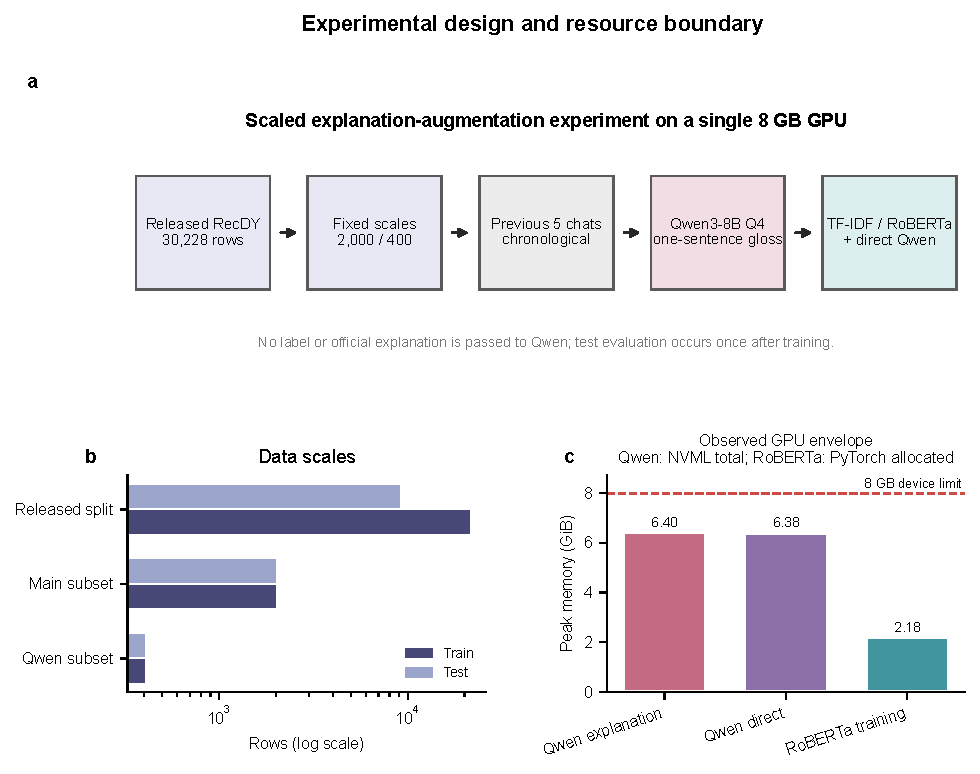
\includegraphics[width=\textwidth]{fig1_workflow.pdf}
  \caption{缩小复现实验流程与资源边界。上方为数据、上下文、Qwen 释义和分类器的执行顺序；下方给出三层数据规模及实测显存。Qwen 显存为 NVML 的整卡使用量，RoBERTa 为 PyTorch allocator 的峰值，二者计量口径不同。}
  \label{fig:workflow}
\end{figure}

\FloatBarrier

\section{方法}

\subsection{本地 Qwen3-8B 解释生成}

Qwen3 技术报告描述了 dense/MoE 系列、思考与非思考双模式以及多语言能力\cite{yang2025qwen3}。本实验使用 Ollama 的 \texttt{qwen3:8b}，参数规模 8.2B，量化格式 Q4\_K\_M。为控制 8 GB 显存和输出稳定性，设置 temperature 0、\texttt{num\_ctx=1024}、\texttt{num\_predict=96}、batch size 1，并以 \texttt{/no\_think} 关闭展开的思考输出。每个样本输入仅包括当前弹幕和真实此前 5 条；不传入标签，也不传入仓库官方释义。

生成目标为一句现代汉语释义：
\begin{equation}
  \widehat E_i = G_{\text{Qwen3-8B-Q4}}(C_i,H_i^{(5)}),
\end{equation}
并将下游输入写为 $X_i=[C_i;\widehat E_i]$。本地窗口 5 小于论文窗口 20，是显式的算力缩小设置；本地提示也强调通用语义释义，而论文官方背景使用不同生成模型和更强购买任务先验，故两种解释源不可用于纯模型优劣归因。

\subsection{输入条件与消融}

在同一 400/400 行上比较以下条件：

\begin{enumerate}[leftmargin=2em]
  \item \textbf{Current：}仅当前弹幕 $C_i$；
  \item \textbf{Raw Context：}当前弹幕与原始此前 5 条 $[C_i;H_i^{(5)}]$；
  \item \textbf{Qwen Explanation：}当前弹幕与本地释义 $[C_i;\widehat E_i]$；
  \item \textbf{Official Explanation：}当前弹幕与仓库官方释义 $[C_i;E_i^{\mathrm{official}}]$；
  \item \textbf{Qwen Direct：}Qwen3-8B 直接依据当前弹幕和前 5 条输出数字 0 或 1。
\end{enumerate}

Raw Context 是关键归因对照：若没有它，Current 到 Qwen Explanation 的变化同时混合“获得上下文”与“LLM 压缩解释”两种效应，无法判断收益来自信息增加还是语义压缩。

\subsection{字符 TF--IDF 与逻辑回归}

第一类分类器采用字符 1--4 gram TF--IDF，\texttt{min\_df=2}、最多 100,000 个特征、sublinear TF；分类头为 class-balanced Logistic Regression，$C=4$、\texttt{liblinear}、最多 1,000 次迭代。TF--IDF 是经典文本表示\cite{manning2008information}，二元 Logistic Regression 的统计基础可追溯至 Cox\cite{cox1958binary}。该模型训练快、行为透明，适合作为完整发布划分与解释输入的低成本敏感性探针。

\subsection{Chinese-RoBERTa 微调}

第二类分类器为 \texttt{hfl/chinese-roberta-wwm-ext}，其中文预训练资源与 whole-word masking 依据见\cite{cui2020revisiting,cui2021wholeword}；RoBERTa 的训练优化思想见\cite{liu2019roberta}。本地实现使用完整参数微调而非 LoRA：102,269,186 个可训练参数，学习率 $4\times10^{-5}$，weight decay 0.01，线性调度和 10\% warmup，max length 128，物理 batch 8、梯度累积 2、有效 batch 16，FP16，固定 3 epochs。随机种子为 100、101、102，报告 mean$\pm$SD。测试集只在每次训练结束后评估一次，不据测试结果挑选 epoch。

\subsection{评价指标与统计方法}

报告 Accuracy、正类 Precision/Recall/F1 以及 Macro-Precision、Macro-Recall、Macro-F1。正文主表以 Macro 指标为主，避免 60.7\% 正类比例掩盖闲聊类表现。对类别 $c\in\{0,1\}$，有
\begin{equation}
  F1_c=\frac{2P_cR_c}{P_c+R_c},\qquad
  \mathrm{MacroF1}=\frac{F1_0+F1_1}{2}.
\end{equation}

TF--IDF 的绝对指标区间由行级非参数 bootstrap 得到\cite{efron1979bootstrap,efron1986bootstrapci}；条件差异使用同一测试行的 5,000 次配对 bootstrap，报告百分点差和 percentile 95\% CI。由于行嵌套在仅 12 个直播间内，该区间忽略群集相关，仅作为探索性不确定性描述，不能代替按直播间聚类或外部直播间验证。

\subsection{本地软硬件环境}

本地工作站为 Intel Core i7-14650HX、31.74 GB RAM、RTX 4060 Laptop GPU（8,188 MiB），驱动 591.86。RoBERTa 环境为 Python 3.13.9、PyTorch 2.12.0+cu126、Transformers 5.0.0；大模型由 Ollama 0.7.1 提供本地 API。LaTeX 使用 TeX Live 2025 XeLaTeX。环境快照保存在 \path{experiment/results/environment.json}。

\section{实验结果}

\subsection{RQ1：8 GB 显存下的大模型可运行性}

表2给出 Qwen 运行结果。800 条释义成功率为 100\%，训练与测试两部分合计端到端耗时 \QwenGenerationWallSeconds\,s；逐条平均约 \QwenGenerationMeanSeconds\,s，峰值整卡显存 \QwenGenerationPeakGiB\,GiB。直接分类 400 条也全部解析成功，覆盖率 \QwenDirectCoverage\%，平均 \QwenDirectMeanSeconds\,s/条。由此可确认 Q4\_K\_M 量化的 8.2B 模型在该 8 GB GPU 上具有稳定实验可行性。

\begin{table}[htbp]
\centering
\caption{Qwen3-8B 本地推理效率。峰值显存为 NVML 整卡用量。}
\label{tab:efficiency}
\begin{tabular}{lrrrrr}
\toprule
阶段 & 请求数 & 成功数 & 平均 s/条 & 墙钟时间/s & 峰值/GiB \\
\midrule
训练集释义 & 400 & 400 & 0.568 & 227.3 & 6.40 \\ 
测试集释义 & 400 & 400 & 0.557 & 222.9 & 6.39 \\ 
Qwen直接分类 & 400 & 400 & 0.209 & 83.8 & 6.38 \\ 
\bottomrule
\end{tabular}

\end{table}

\subsection{RQ2：解释压缩与原始上下文的差异}

完整指标见表~\ref{tab:classical} 和图~\ref{fig:classical}。在 Full 设置中，当前弹幕+官方释义的 Macro-F1 为 \FullOfficialMacroF\%，高于仅当前弹幕的 \FullContentMacroF\%；增量 \FullOfficialDeltaPP\ 个百分点的 95\% 配对区间不含 0。仅使用官方释义反而略弱于仅弹幕，说明释义并非替代原文，而是作为补充信息更合适。

在 400/400 设置中，本地 Qwen 释义得到 \SmallQwenMacroF\%，相对仅弹幕 \SmallContentMacroF\% 提高 \SmallQwenDeltaPP\ 个百分点；但 95\% CI [\SmallQwenDeltaLowPP, \SmallQwenDeltaHighPP] 跨过 0，因此应表述为正向趋势，而非确定改善。仓库官方释义达到 \SmallOfficialMacroF\%，同样因样本量小而区间跨 0。直接拼接原始前 5 条只有 \SmallRawMacroF\%，相对基线下降 \SmallRawDeltaPP\ 个百分点，说明未压缩上下文引入了大量干扰特征。

\begin{table}[htbp]
\centering
\caption{字符 TF--IDF + Logistic Regression 的主要结果（\%）。P/R/F1 均为 Macro 口径。}
\label{tab:classical}
\input{table_classical.tex}
\end{table}

\begin{table}[htbp]
\centering
\caption{相对“仅当前弹幕”的 Macro-F1 配对效应（百分点）。CI 为 5,000 次行级配对 bootstrap。}
\label{tab:bootstrap}
\begin{tabular}{lrrr}
\toprule
比较条件 & 差值/pp & 95\% CI/pp & 测试行数 \\
\midrule
Full: +官方释义 & 1.26 & [0.58, 1.94] & 9,069 \\
2,000: +官方释义 & 3.31 & [1.54, 5.09] & 2,000 \\
400: +原始前5条 & -17.19 & [-22.75, -11.76] & 400 \\
400: +Qwen释义 & 1.87 & [-2.80, 6.69] & 400 \\
400: +官方释义 & 3.03 & [-1.78, 7.71] & 400 \\
\bottomrule
\end{tabular}

\end{table}

\begin{figure}[htbp]
  \centering
  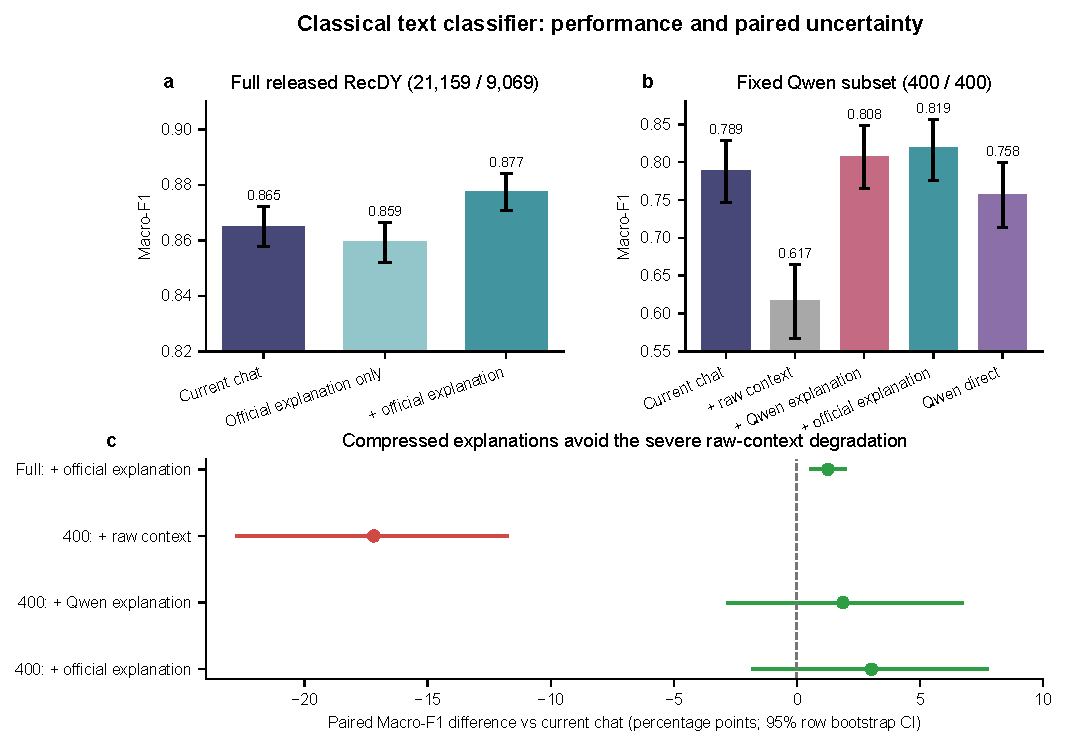
\includegraphics[width=\textwidth]{fig2_classical_results.pdf}
  \caption{字符 TF--IDF 分类结果。a，完整发布划分的 Macro-F1；b，固定 400/400 子集与 Qwen 直接分类；c，相对仅当前弹幕的配对效应。误差线为 95\% 行级 bootstrap CI。压缩释义避免了原始上下文造成的严重退化，但 400 条设置下释义增量的不确定区间仍包含 0。}
  \label{fig:classical}
\end{figure}

\subsection{RQ3：训练规模与下游模型交互}

Chinese-RoBERTa 的结果与 TF--IDF 不完全相同（表~\ref{tab:roberta}，图~\ref{fig:roberta}）。在 2,000/2,000 设置中，官方释义将 Macro-F1 从 \RobertaMainContentMean$\pm$\RobertaMainContentSD\% 提高到 \RobertaMainOfficialMean$\pm$\RobertaMainOfficialSD\%，三个种子均为正向，平均增量 \RobertaMainDeltaPP\ 个百分点。

然而在 400/400 设置中，仅弹幕已经达到 \RobertaSmallContentMean\%，本地 Qwen 释义为 \RobertaSmallQwenMean\%，平均下降 \RobertaSmallQwenDeltaPP\ 个百分点；三个种子均下降。官方释义和本地释义在这一低数据设置都未超过仅弹幕，而原始上下文进一步大幅下降。该结果表明：解释序列增加了输入长度和可学习模式，在训练样本不足时可能扩大过拟合或解释噪声；只有当训练规模足以学习“何时相信解释”时，增强才可能转化为稳定收益。

\begin{table}[htbp]
\centering
\caption{Chinese-RoBERTa 三随机种子结果（mean$\pm$SD，\%）。}
\label{tab:roberta}
\resizebox{\textwidth}{!}{\begin{tabular}{llrrrr}
\toprule
训练规模 & 输入条件 & Accuracy & Macro-P & Macro-R & Macro-F1 \\
\midrule
2,000 & 仅当前弹幕 & 87.83$\pm$0.43 & 87.49$\pm$0.55 & 86.92$\pm$0.54 & 87.16$\pm$0.45 \\
2,000 & 当前弹幕+官方释义 & 89.03$\pm$0.08 & 89.23$\pm$0.11 & 87.66$\pm$0.09 & 88.30$\pm$0.08 \\
400 & 仅当前弹幕 & 85.83$\pm$1.42 & 85.63$\pm$1.54 & 84.40$\pm$1.50 & 84.90$\pm$1.52 \\
400 & 当前弹幕+原始前5条 & 72.25$\pm$5.48 & 72.68$\pm$6.52 & 67.43$\pm$6.43 & 67.69$\pm$7.28 \\
400 & 当前弹幕+Qwen释义 & 83.58$\pm$0.38 & 83.16$\pm$0.37 & 82.24$\pm$1.08 & 82.57$\pm$0.67 \\
400 & 当前弹幕+官方释义 & 84.17$\pm$1.38 & 84.37$\pm$0.83 & 82.23$\pm$2.24 & 82.91$\pm$1.86 \\
\bottomrule
\end{tabular}
}
\end{table}

\begin{figure}[htbp]
  \centering
  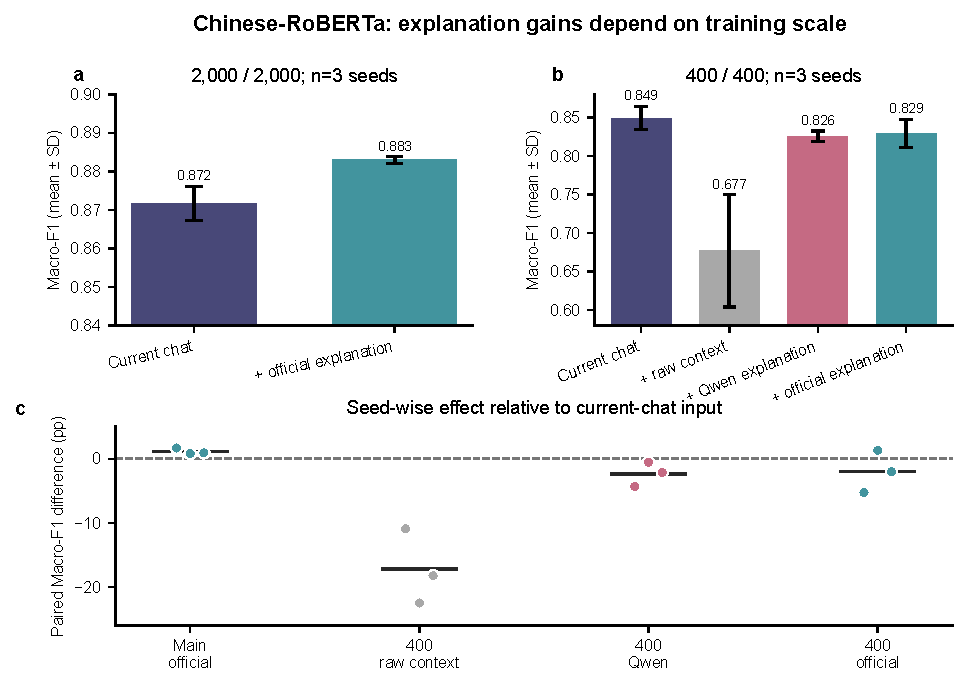
\includegraphics[width=\textwidth]{fig3_roberta_results.pdf}
  \caption{Chinese-RoBERTa 的规模效应。a，2,000/2,000 设置下官方释义产生一致小幅增益；b，400/400 设置下原始上下文和两种释义均未超过仅弹幕；c，三个随机种子的配对 Macro-F1 差。误差线为种子间 SD，不是置信区间。}
  \label{fig:roberta}
\end{figure}

\subsection{RQ4：直接分类还是解释器}

Qwen3-8B 直接分类的 Macro-F1 为 \SmallDirectMacroF\%，低于同一 400 条测试集上的 TF--IDF 仅弹幕（\SmallContentMacroF\%）和 TF--IDF+Qwen 释义（\SmallQwenMacroF\%）。尽管直接分类更快（\QwenDirectMeanSeconds\,s/条），它没有利用 400 条带标签训练样本。当前证据因此更支持“Qwen 负责语义压缩，小模型负责监督判别”的混合角色，而不是让 8B 模型在零样本下替代监督分类器。

\subsection{资源与文本特征}

本地 Qwen 释义平均 21.72 个汉字，短于仓库官方释义的 37.54 个汉字，但长于原弹幕的 8.43 个汉字。图~\ref{fig:efficiency} 汇总了逐条延迟、阶段总时间、显存和文本长度。Qwen 解释生成与直接分类的峰值整卡显存都约 6.4 GiB；RoBERTa 三轮训练的 PyTorch 分配峰值约 2.2 GiB。由于两种显存计量口径不同，只能分别证明各阶段未越过设备上限，不能用柱高推断框架效率优劣。

\begin{figure}[htbp]
  \centering
  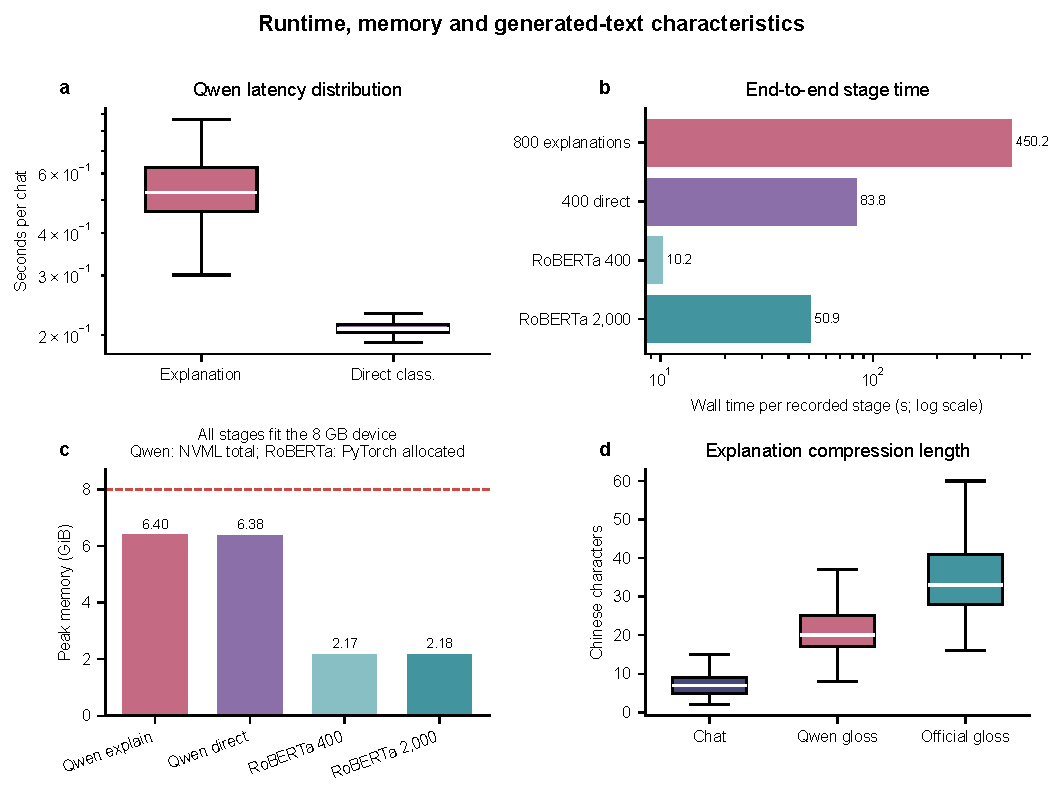
\includegraphics[width=\textwidth]{fig4_efficiency.pdf}
  \caption{运行效率与文本特征。a，Qwen 逐条延迟分布；b，各阶段端到端时间（任务规模不同，不能作等价吞吐比较）；c，峰值显存与 8 GB 设备线；d，原弹幕、本地释义和官方释义的字符长度分布。}
  \label{fig:efficiency}
\end{figure}

\FloatBarrier

\subsection{案例分析}

表~\ref{tab:cases} 展示了本地释义的典型作用。它能把“蓝莓还有吧今天”压缩为明确的库存询问，也能将对主播状态的称赞与购买意图分离；但当上下文指代错误时，也会把“泥膜和控油乳”误解释成生日礼物，或把“把你上架”的玩笑字面化为商品上架。后一类错误与目标论文所讨论的过度解释、局部词依赖和隐含指代问题一致\cite{zhu2026bc4rii}。

\begin{table}[htbp]
\centering
\caption{TF--IDF 条件下的代表性预测翻转。0=闲聊，1=购买。}
\label{tab:cases}
\small
\begin{tabularx}{\textwidth}{p{2.4cm}cXc}
\toprule
当前弹幕 & 金标 & Qwen 释义 & 仅弹幕$\rightarrow$加释义 \\
\midrule
蓝莓还有吧今天 & 1 & 询问今天是否有蓝莓库存。 & $0\rightarrow1$ \\
刘媛媛这个状态真不错 & 0 & 弹幕是在称赞刘媛媛当前的精神状态和表现。 & $1\rightarrow0$ \\
泥膜和控油乳 & 1 & 当前弹幕是在补充说明之前提到的生日礼物，表示收到的礼物中还包括泥膜和控油乳。 & $1\rightarrow0$ \\
把你上架 & 0 & 弹幕希望主播将商品上架。 & $0\rightarrow1$ \\
\bottomrule
\end{tabularx}
\end{table}

另一个值得警惕的样本是“已拍加急”：文本和两种释义都指向已下单，但仓库金标为 0。该现象可能来自语境标注规则、说话对象或噪声，说明错误并不全由模型造成。当前实验没有重新人工标注，因而不对标签质量作总体推断。

\section{改进方法与改进前后对比}

\subsection{改进动机与预注册假设}

首轮实验暴露了两个相互独立的问题。第一，通用的一句话释义虽然比原始前文更紧凑，但结构化提示词生成的“原句证据”有时会重复或幻觉式扩展当前弹幕；第二，将当前弹幕和释义等权拼接到 RoBERTa 输入中，无法保证模型学习到何时信任释义。因而本节预先固定两个改进假设：

\begin{enumerate}[leftmargin=2em]
  \item 将解释压缩为“对象+言语行为”，去掉可能重复当前文本的证据字段，可减少输入噪声；
  \item 内容分支和解释分支分别学习，再用训练集内部验证选择概率融合权重与决策阈值，比直接拼接更稳健。
\end{enumerate}

改进实验不重新抽取测试样本。400 条测试集的 \texttt{row\_id}、标签和真实前文保持不变；新增 1,000 条训练集是原 400 条训练集的嵌套扩展。结构化 Qwen 解释覆盖率为训练 400 条的 \ImproveQwenTrainSmallCoverage\%、训练 1,000 条的 \ImproveQwenTrainLargeCoverage\% 和测试集的 \ImproveQwenTestSmallCoverage\%。失败样本不使用真实标签修补，并在结果目录中保留原始响应。

\subsection{结构化解释与紧凑输入}

结构化提示词要求 Qwen 只输出“对象；言语行为；原句证据”，当前弹幕优先，前文仅作指代消歧，不输出类别或购买意图判断。RoBERTa 的紧凑输入进一步只保留对象和言语行为，形成
\begin{equation}
  X_t = [\text{当前弹幕}]\;\texttt{[SEP]}\;[\text{对象；言语行为}].
\end{equation}
这一步不重新调用 Qwen，也不使用标签筛选文本，因此可以单独检验“去除证据字段”这一表示改动。

\subsection{训练集内部晚期融合}

对 TF--IDF，内容和解释分别训练字符 $n$-gram + Logistic Regression，在训练集上做 5 折 OOF 预测；网格搜索 $\alpha\in\{0,0.05,\ldots,1\}$ 和阈值 $\tau\in[0.40,0.60]$，只用 OOF Macro-F1 选择参数。RoBERTa 采用相同思想，但使用固定 20\% 训练内部验证集：分别训练内容模型和紧凑解释模型，在验证集选择 $\alpha$ 与 $\tau$，随后用完整训练集重训两个分支，测试集只做最终推理。所有种子均为 100、101、102，未根据测试集最高分挑选表示或阈值。

\begin{table}[htbp]
\centering
\caption{改进前后 TF--IDF 结果。晚期融合的参数只由训练集 OOF 选择。}
\label{tab:improvement-classical}
\resizebox{\textwidth}{!}{\begin{tabular}{llrrr}
\toprule
规模 & 条件 & Macro-F1 & 相对当前弹幕 & 选择方式\\
\midrule
400/400 & 当前弹幕 & 78.88\% & +0.00\,pp & 固定\\
400/400 & 旧提示词拼接 & 80.75\% & +1.87\,pp & 固定\\
400/400 & 结构化提示词拼接 & 80.84\% & +1.96\,pp & 固定\\
400/400 & 旧提示词晚期融合 & 82.39\% & +3.51\,pp & OOF\\
400/400 & 结构化晚期融合 & 80.03\% & +1.14\,pp & OOF\\
\addlinespace
1000/400 & 当前弹幕 & 82.29\% & +0.00\,pp & 固定\\
1000/400 & 结构化提示词拼接 & 82.94\% & +0.65\,pp & 固定\\
1000/400 & 结构化晚期融合 & 83.82\% & +1.53\,pp & OOF\\
\bottomrule
\end{tabular}
}
\end{table}

\subsection{结果：经典分类器获得更稳定的收益}

在 400/400 设置中，旧提示词的 OOF 晚期融合将 Macro-F1 从 \ImproveTFIDFSmallContent\% 提高到 \ImproveTFIDFSmallOldLate\%，点增量为 \ImproveTFIDFSmallOldLateDeltaPP\ 个百分点，行级 95\% CI 为 [\ImproveTFIDFSmallOldLateLowPP,\,\ImproveTFIDFSmallOldLateHighPP]。区间仍跨过 0，因此这里称为探索性提升；但它明确优于固定拼接的点估计，说明融合方式本身比继续堆叠文本更有希望。

在嵌套的 1,000/400 设置中，结构化释义拼接得到 \ImproveTFIDFLargeStructuredConcat\%，晚期融合得到 \ImproveTFIDFLargeStructuredLate\%，相对同规模当前弹幕提高 \ImproveTFIDFLargeLateDeltaPP\ 个百分点，行级 95\% CI 为 [\ImproveTFIDFLargeLateLowPP,\,\ImproveTFIDFLargeLateHighPP]。这组结果支持“增加训练样本并让分类器学习如何加权解释”这一组合方向，但由于测试集仍只有 400 行和 12 个直播间，不能视为已确证的泛化提升。

\subsection{结果：RoBERTa 的负结果被部分修复}

直接把完整结构化字符串拼接到 RoBERTa 并没有改善结果：1,000 条训练时 Macro-F1 为 \ImproveRobertaLargeStructured\%。去掉证据字段后的紧凑表示提高到 \ImproveRobertaLargeCompact\%，再进行验证集晚期融合后达到 \ImproveRobertaLargeLateFusion\%，相对纯当前弹幕 \ImproveRobertaLargeContent\% 的点增量为 \ImproveRobertaLargeLateDeltaPP\ 个百分点；三个种子的标准差也从紧凑拼接的约 0.51 个百分点降至约 0.29 个百分点。400 条设置下，晚期融合为 \ImproveRobertaSmallLateFusion\%，与纯内容 \ImproveRobertaSmallContent\% 基本持平，但高于原始 Qwen 拼接的 \ImproveRobertaSmallOldQwen\%。

这说明首轮 RoBERTa 下降并不完全来自“解释没有信息”，而部分来自证据重复、输入拼接和决策阈值未校准。与此同时，400 条设置没有得到可靠的正向区间，不能把紧凑表示写成普遍有效的解决方案。改进的主要证据是 1,000 条设置下的点估计和更小的种子间波动，而不是测试集显著性检验。

\begin{table}[H]
\centering
\small
\caption{RoBERTa 紧凑表示与验证集晚期融合结果（mean$\pm$SD，\%）。}
\label{tab:improvement-roberta}
\begin{tabular}{lrrr}
\toprule
条件 & 训练条数 & Macro-F1 & SD\\
\midrule
400 当前弹幕 & 400 & 84.90\% & 1.52\%\\
400 旧 Qwen 拼接 & 400 & 82.57\% & 0.67\%\\
400 结构化拼接 & 400 & 82.44\% & 1.66\%\\
400 紧凑拼接 & 400 & 84.30\% & 1.75\%\\
400 紧凑晚期融合 & 400 & 84.88\% & 0.61\%\\
1000 当前弹幕 & 1000 & 87.19\% & 0.53\%\\
1000 结构化拼接 & 1000 & 86.73\% & 1.12\%\\
1000 紧凑拼接 & 1000 & 87.21\% & 0.51\%\\
1000 紧凑晚期融合 & 1000 & 87.63\% & 0.29\%\\
\bottomrule
\end{tabular}

\end{table}

\subsection{归因、成本与失败案例}

2$\times$2 TF--IDF 对照显示：旧提示词从拼接改为晚期融合带来正向变化，而结构化提示词本身相对旧提示词拼接几乎没有增量；结构化提示词与晚期融合组合在 400 条上反而低于旧提示词晚期融合。因此，当前证据支持的是“表示压缩 + 训练内融合”的系统级改进，不支持“结构化提示词单独优于通用提示词”的结论。

结构化 Qwen 生成仍是主要成本：400 条训练加测试约 714 s，1,000 条训练加同一测试约 1,274 s；RoBERTa 晚期融合的单组记录时间约 19 s（400 条）和 47 s（1,000 条），峰值显存约 2.2 GiB。1,000 条训练集有 3 条、测试集有 2 条响应因证据字段超出当前弹幕而未通过结构校验，恰好说明证据约束是必要的；这些响应没有被改写成成功样本，400 条嵌套训练集中的 1 条失败也包含在上述训练计数内。

\begin{figure}[H]
  \centering
  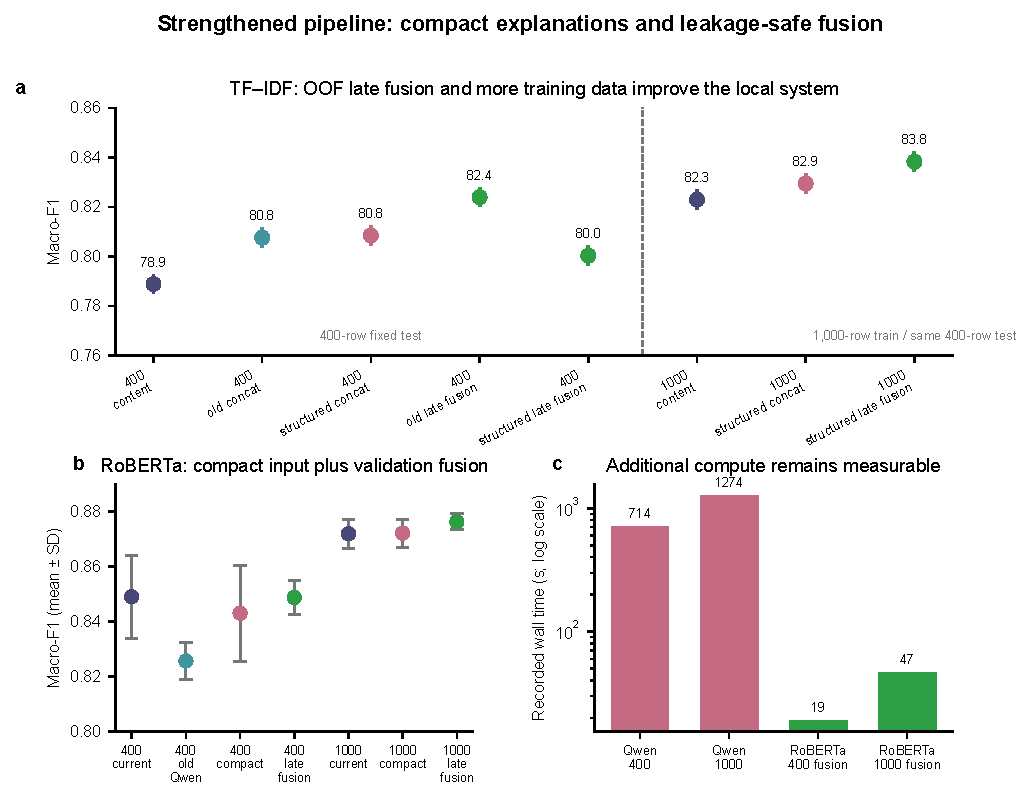
\includegraphics[width=0.92\textwidth]{fig5_improvement_results.pdf}
  \caption{改进实验的定量对比。a，TF--IDF 在固定 400 条测试集上的两种训练规模与晚期融合条件；b，RoBERTa 三个随机种子的均值和标准差，紧凑表示去掉了重复证据字段，晚期融合进一步用训练内部验证选择权重；c，Qwen 生成与 RoBERTa 融合的记录墙钟时间。}
  \label{fig:improvement}
\end{figure}

\begin{keybox}[本轮改进的结论边界]
本轮最可靠的工程改进是：在 4060 上保留 Qwen 作为离线语义压缩器，用紧凑对象--行为字段作为辅助输入，并在训练内部验证集上学习融合权重。它在 1,000 条设置下使 TF--IDF 达到 \ImproveTFIDFLargeStructuredLate\%，使 RoBERTa 达到 \ImproveRobertaLargeLateFusion\%；但 400 条规模的区间仍不确定，且完整 SPT--RII 仍未复现。
\end{keybox}

\section{讨论}

\subsection{解释的作用更接近选择性压缩，而非简单扩充}

Raw Context 在 TF--IDF 和 RoBERTa 上都显著退化，说明“更多文本”并不等于“更多有效信息”。前 5 条可能涉及不同商品、问候或主播互动；字符 n-gram 会直接吸收这些词，预训练模型在仅 400 条监督数据时也难以学会忽略。相比之下，一句话释义将多条输入压缩为一个面向当前弹幕的语义假设，至少避免了原始拼接的严重退化。这是本实验最稳定的机制性观察，但它仍是行为证据，不证明模型内部形成了特定因果机制。

\subsection{小规模下的负结果是有用结论}

本地 Qwen 释义对 TF--IDF 呈正向趋势，却对 400 条 RoBERTa 稳定负向。若只报告最佳条件，会错误得出“LLM 解释必然增强分类”的结论。更合理的解释是：线性模型从规范化的释义词汇中直接获益，而高容量 RoBERTa 在低数据下可能同时拟合弹幕和解释中的偏差。改进实验进一步表明，去掉重复证据字段并在验证集校准融合后，1,000 条 RoBERTa 的 Macro-F1 可回升到 \ImproveRobertaLargeLateFusion\%，但 400 条设置仍未超过纯内容基线；因此，样本规模和融合策略是负结果的重要调节因素，而不是可以忽略的实现细节。

\subsection{紧凑表示与验证集融合修复了部分退化}

把结构化解释拆成对象和言语行为后，RoBERTa 在 1,000 条设置中由 \ImproveRobertaLargeStructured\% 提高到 \ImproveRobertaLargeCompact\%；再用训练内部验证集选择分支权重和阈值，达到 \ImproveRobertaLargeLateFusion\%。这种改进没有改变 Qwen 模型，也没有使用测试标签，说明首轮退化的一部分来自表示冗余和未经校准的等权拼接。400 条设置的晚期融合结果为 \ImproveRobertaSmallLateFusion\%，与 \ImproveRobertaSmallContent\% 基本持平，仍应视为恢复而非确证的增益。

\subsection{本地 Qwen 与官方释义不可作纯模型比较}

目标论文 Table 9 使用 Qwen2.5-7B、Llama3.1-8B 和 DeepSeek-V3 比较解释生成，并在 RTX 4090 上报告 Qwen2.5-7B 约 283 ms/条；本地实验使用 Qwen3-8B Q4、窗口 5 和不同提示，约 \QwenGenerationMeanSeconds\,s/条。因此，官方释义比本地释义更长、部分分类结果更好，可能同时来自窗口 20、生成模型、提示任务先验和后处理差异。报告只将两者称为“不同解释源”，不归因于 Qwen3 与某一官方模型的纯性能差。

\subsection{与原论文结论的关系}

原论文的 SPT-RII 还包含 soft prompt 和动态词表，其 RecDY 50--70 shot 主表 F1 约 77.84--79.23。当前本地监督结果使用 400、2,000 或 21,159 条训练、不同分类头与不同指标实现，不能与这些数值作同条件排名。当前结果只支持原论文一个较窄的思想：短弹幕可能受益于语境解释；同时补充了一个重要边界，即在低数据和高容量下游模型中，解释也可能成为噪声源。

\section{有效性威胁与局限}

\begin{enumerate}[leftmargin=2em,label=\arabic*.]
  \item \textbf{同直播间行级划分。} 训练和测试的 12 个 \texttt{live\_id} 完全重合，因此不能声称对未见主播或未见直播间泛化。
  \item \textbf{文本重复。} Full 测试中有 \ContentOverlapPct\% 的 \texttt{content} 在训练中出现；五字段完全相同的测试行有 \ExactOverlapRows\ 条。Main 的五字段重复仅 1/2,000，Qwen 子集为 0，但域内重复仍可能抬高 Full 指标。
  \item \textbf{传导式上下文。} 真实前文重建使用另一划分的未标注文本，符合在线连续流但不符合严格归纳评测。后续应按时间或直播间划分后重新生成解释。
  \item \textbf{行级 bootstrap。} 当前区间未对直播间内相关性聚类；只有 12 个直播间时，群集 bootstrap 的有效样本量也有限。
  \item \textbf{解释质量未人工评分。} 目前仅用下游分类和长度衡量解释，没有对忠实性、指代正确性和幻觉率进行盲评。
  \item \textbf{缩小实现不含 SPT-RII 全部模块。} 动态 verbalizer 和 soft prompt 尚未复现，不能将本地结果写成 SPT-RII 主表复现。
  \item \textbf{单数据源、单设备。} 当前仅 RecDY、单张 4060 和一个 Qwen 量化版本；没有跨 RecKS、RecXHS、RecTikTok 或不同显卡验证。
  \item \textbf{数据与论文口径不完全一致。} 仓库带解释数据 96,243 条与论文总量 143,957 条之间缺少公开过滤说明，限制了完整可追溯性。
\end{enumerate}

\section{下一步研究计划}

按照“先完成可运行实验，再逐步提高研究质量”的顺序，改进实验已经完成紧凑表示、训练规模扩展和训练内融合；下一阶段重点转向外部有效性与解释质量：

\begin{enumerate}[leftmargin=2em]
  \item \textbf{严格划分。} 以直播间留一或按时间前 70\%/后 30\% 划分，在划分后只使用过去可见文本生成解释，重新评估跨直播间和时间漂移。
  \item \textbf{窗口与提示联合消融。} 在同一测试行上比较 $k\in\{0,5,10,20\}$ 与通用/结构化输出，继续使用训练内融合选择规则。
  \item \textbf{更完整的样本量曲线。} 在当前 400 和 1,000 条结果基础上扩展到 2,000 条，定位解释从噪声转为增益的临界区域。
  \item \textbf{人工解释审计。} 对随机 200 条进行双人盲评，评价忠实性、指代正确、过度解释和标签诱导，并报告一致性系数。
  \item \textbf{逐步靠近 SPT-RII。} 先补齐官方数据处理器和模板消融，再实现动态 verbalizer；每新增模块都保留 Current、Raw Context 和 Explanation 三个对照。
\end{enumerate}

\section{结论}

本研究在 RTX 4060 Laptop GPU 8 GB 上完成了与 BC4RII 相关的解释增强缩小实验、官方仓库审计和完整复现性记录。Qwen3-8B Q4 能以约 \QwenGenerationMeanSeconds\,s/条稳定生成一句话释义，峰值整卡显存约 \QwenGenerationPeakGiB\,GiB，证明本地 8B 解释器具有现实可操作性。实验最稳健的发现不是“解释总能提高分类”，而是原始上下文直接拼接会严重干扰分类，语义压缩能够避免这种退化；至于是否超过仅当前弹幕，则取决于解释源、表示方式、融合策略、训练规模和下游模型。改进后的 TF--IDF 在 1,000 条设置达到 \ImproveTFIDFLargeStructuredLate\%，RoBERTa 经紧凑表示和验证集晚期融合达到 \ImproveRobertaLargeLateFusion\%，但 400 条设置仍只有恢复性结果。因而，下一步研究应把重点从“换更大的模型”转向严格划分、解释忠实性、窗口/提示消融、聚类级统计和更完整的样本量曲线。

\clearpage
\appendix

\section{Qwen 提示模板}

\subsection{解释生成提示}

\begin{tcolorbox}[breakable,colback=gray!3,colframe=gray!45,title=生成提示（标签不进入提示）]
你是电商直播弹幕语义分析助手。请结合前文，用一句自然的现代汉语解释当前弹幕的真实意图。\\
要求：不要判断或输出分类标签，不要重复原句，不要展示推理过程，不要添加解释以外的内容。\\
前文弹幕：\{此前 5 条，以分号连接\}\\
当前弹幕：\{当前文本\}\\
只输出一句语境释义。\texttt{/no\_think}
\end{tcolorbox}

\subsection{结构化解释提示（structured\_v2）}

\begin{tcolorbox}[breakable,colback=gray!3,colframe=gray!45,title=证据约束提示（不输入标签或官方释义）]
你是电商直播弹幕语义分析助手。请只分析当前弹幕，前文仅用于解析当前弹幕中的指代；如果前文无关，请忽略它。不要判断购买意图，不要输出二分类标签，不要猜测用户没有说出的信息，不要展示推理过程。\\
严格只输出一行：对象：\{对象\}；言语行为：\{言语行为\}；原句证据：\{当前弹幕中的连续原文片段\}。对象和言语行为使用简短中文短语；原句证据必须逐字来自当前弹幕。\\
前文：\{此前 5 条\}\quad 当前弹幕：\{当前文本\}\quad\texttt{/no\_think}
\end{tcolorbox}

\subsection{直接分类提示}

\begin{tcolorbox}[breakable,colback=gray!3,colframe=gray!45,title=零样本分类提示]
判断当前电商直播弹幕是否表达购买或推荐需求。\\
标签 0：闲聊、称赞主播、与商品购买无关的表达。\\
标签 1：询问商品、价格、尺寸、库存、优惠、使用方式，要求展示或表达购买兴趣。\\
前文：\{此前 5 条\}\\
当前弹幕：\{当前文本\}\\
只输出数字 0 或 1，不要解释。\texttt{/no\_think}
\end{tcolorbox}

\section{关键复现实验命令}

所有命令在项目根目录 \path{E:\Lab} 下运行。RoBERTa 使用 \path{D:\Anaconda3\python.exe}；Qwen 与字符基线使用 \texttt{lora\_env}。

\begin{lstlisting}[language={},caption={数据准备与基线}]
D:\Anaconda3\python.exe experiment\src\prepare_data.py
D:\Anaconda3\envs\lora_env\python.exe experiment\src\run_classical.py --suite full
D:\Anaconda3\envs\lora_env\python.exe experiment\src\run_classical.py --suite main
\end{lstlisting}

\begin{lstlisting}[language={},caption={改进实验：固定数据、结构化释义与 OOF 融合}]
D:\Anaconda3\python.exe experiment\src\prepare_improvement_data.py
D:\Anaconda3\envs\lora_env\python.exe experiment\src\generate_improvement_qwen.py --split train --size 400
D:\Anaconda3\envs\lora_env\python.exe experiment\src\generate_improvement_qwen.py --split train --size 1000
D:\Anaconda3\envs\lora_env\python.exe experiment\src\generate_improvement_qwen.py --split test --size 400
D:\Anaconda3\envs\lora_env\python.exe experiment\src\run_improvement_classical.py --sizes 400 1000
D:\Anaconda3\python.exe experiment\src\make_compact_explanations.py
D:\Anaconda3\python.exe experiment\src\train_improvement_roberta.py `
  --train-file improvement\douyin_train_improvement1000_compact_object_act_v1.csv `
  --test-file improvement\douyin_test_improvement400_compact_object_act_v1.csv `
  --tag qwen1000_compact_concat --condition qwen --qwen-column qwen_background_compact `
  --seeds 100 101 102 --epochs 3 --batch-size 8 --accumulation-steps 2 --max-length 128
D:\Anaconda3\python.exe experiment\src\train_roberta_late_fusion.py `
  --train-file improvement\douyin_train_improvement1000_compact_object_act_v1.csv `
  --test-file improvement\douyin_test_improvement400_compact_object_act_v1.csv `
  --tag qwen1000_compact_late_fusion --qwen-column qwen_background_compact `
  --seeds 100 101 102 --epochs 3 --batch-size 8 --accumulation-steps 2 --max-length 128
D:\Anaconda3\python.exe experiment\src\analyze_improvement.py
D:\Anaconda3\python.exe experiment\src\make_improvement_assets.py
\end{lstlisting}

\begin{lstlisting}[language={},caption={Qwen 解释、直接分类与 400 条消融}]
D:\Anaconda3\envs\lora_env\python.exe experiment\src\generate_qwen.py --split train
D:\Anaconda3\envs\lora_env\python.exe experiment\src\generate_qwen.py --split test
D:\Anaconda3\envs\lora_env\python.exe experiment\src\classify_qwen.py
D:\Anaconda3\envs\lora_env\python.exe experiment\src\run_classical.py --suite qwen
\end{lstlisting}

\begin{lstlisting}[language={},caption={RoBERTa 三随机种子示例}]
$env:HF_HOME='D:\hf'
$env:HF_HUB_OFFLINE='1'
D:\Anaconda3\python.exe experiment\src\train_roberta.py `
  --suite main --condition official --seeds 100 101 102 `
  --epochs 3 --batch-size 8 --accumulation-steps 2 --max-length 128
\end{lstlisting}

\begin{lstlisting}[language={},caption={汇总、选例、出图与环境快照}]
D:\Anaconda3\python.exe experiment\src\analyze_results.py
D:\Anaconda3\python.exe experiment\src\select_case_studies.py
D:\Anaconda3\python.exe experiment\src\make_figures.py
D:\Anaconda3\python.exe experiment\src\collect_environment.py
D:\Anaconda3\python.exe experiment\src\make_report_assets.py
\end{lstlisting}

\section{官方仓库代码审计摘要}

\begin{longtable}{p{3.2cm}p{5.2cm}p{6.2cm}}
\caption{官方仓库中影响原样运行和结果解释的主要问题。}\label{tab:repo-audit}\\
\toprule
类别 & 观察 & 本实验处理 \\
\midrule
\endfirsthead
\toprule
类别 & 观察 & 本实验处理 \\
\midrule
\endhead
数据处理器 & \texttt{RecdyProcessor}、\texttt{RelatedProcessor} 未随仓库发布 & 不修改 site-packages，重写显式 CSV 读取与验证 \\
模型路径 & 多处为作者 \texttt{/home/...} 绝对路径 & 使用 Hugging Face 缓存和相对项目路径 \\
依赖 & requirements 含 Linux CUDA/NCCL/Triton 与占位包 & 使用已验证的 Windows CUDA PyTorch 环境和最小依赖 \\
批次错误 & \texttt{autorun.py} 最后一批读取 \texttt{row[1]}，弹幕应为 \texttt{row[2]} & 不调用该入口；以字段名读取 \\
梯度累积 & 官方参数只影响 scheduler，未真正累积梯度 & 本地每 $k$ 步 optimizer step，有效 batch 明确记录 \\
测试模式 & 零样本脚本缺少 \texttt{eval()} 与 \texttt{no\_grad()} & 本地推理关闭梯度；RoBERTa 测试只执行一次 \\
checkpoint & 多随机种子共享路径，可能互相覆盖 & 每个 suite/condition/seed 独立 JSON 与预测文件 \\
数据口径 & 带解释文件 96,243 条，少于论文 143,957 条 & 报告明确限定为仓库带解释 RecDY 子集 \\
\bottomrule
\end{longtable}

\section{结果与文件清单}

\begin{longtable}{p{5.2cm}p{9.4cm}}
\toprule
路径 & 内容 \\
\midrule
\endfirsthead
\toprule
路径 & 内容 \\
\midrule
\endhead
\path{experiment/data/processed/} & 固定 full/main/qwen 数据、真实上下文和 Qwen 释义；\texttt{improvement/} 含嵌套的 400/1,000 训练集 \\
\path{experiment/logs/} & Qwen 逐条 JSONL 断点日志，含输入哈希、提示词版本、延迟、token 数和错误 \\
\path{experiment/results/} & 每个分类条件的 JSON、逐行预测、配对 bootstrap、环境和数据审计；\texttt{improvement/} 含 OOF 选择记录 \\
\path{experiment/figures/} & 五张主图的 SVG/PDF/PNG/TIFF 与 source-data CSV \\
\path{experiment/src/train\_roberta\_late\_fusion.py} & 训练内部验证集选权重/阈值的 RoBERTa 双分支融合运行器 \\
\path{experiment/archive/invalid_sparse_context_20260718/} & 首轮错误稀疏上下文结果的只读归档，不用于正文 \\
\path{experiment/report/report.tex} & 本报告 LaTeX 源文件 \\
\path{experiment/report/report.pdf} & 编译后的最终报告（含改进章节和图5） \\
\bottomrule
\end{longtable}

\section{论断—证据—边界核对}

\begin{longtable}{p{5.1cm}p{5.4cm}p{4.3cm}}
\toprule
主要论断 & 直接证据 & 边界 \\
\midrule
\endfirsthead
\toprule
主要论断 & 直接证据 & 边界 \\
\midrule
\endhead
4060 8 GB 可运行本地 8B 解释器 & 800/800 成功；峰值 6.40 GiB；逐条日志 & 仅 Q4\_K\_M、batch 1、上下文 1,024 \\
原始上下文直接拼接会干扰分类 & 两种分类器、三个种子均显著/稳定下降 & 仅窗口 5、当前 RecDY 行级划分 \\
本地 Qwen 释义对 TF--IDF 有正向趋势 & Macro-F1 +1.87 pp & 95\% CI 跨 0，不能称显著改善 \\
官方释义在较大训练规模下有小幅收益 & Full TF--IDF CI 不含 0；2,000 RoBERTa 三种子均正向 & 解释源与本地 Qwen 不同，不能纯模型归因 \\
紧凑表示与训练内融合可部分修复 RoBERTa 退化 & 1,000 条：87.19\% 当前、87.21\% 紧凑、87.63\% 晚期融合；验证集选参 & 400 条仍近似持平，测试集仅 400 行 \\
\bottomrule
\end{longtable}

\printbibliography[heading=bibintoc,title={参考文献}]

\end{document}
